
% COURS 1

\section{Théorie des Graphes}

\subsection{Définitions}

\begin{defn}
Un graphe $\Gamma$ est un triplet $(V,E,\gamma)$ où V est un ensemble fini dont les éléments sont appelés sommets, E est un ensemble fini dont les éléments sont appelés arêtes, $\gamma$ est une fonction $\gamma : E \rightarrow Paires(V)$. On notera le plus souvent $\Gamma = (V,E)$ en omettant la fonction $\gamma$.

Soit $\gamma(e) = \{x,y\}$ pour $e \in E, x,y \in V$:
\begin{enumerate}
	\item On dit que x et y sont adjacents.

	\item On dit que e est incidente à x et y. 
\end{enumerate}

\end{defn}

\begin{defn}
Soit $\Gamma = (V,E,\gamma)$ un graphe.

\begin{enumerate}
	\item $\gamma(e)= \{x,x\}$ pour $e \in E, x \in V$ est appelé un lacet.
	\item Si au moins 2 arêtes sont incidentes à 2 mêmes sommets, on les appelle arêtes multiples.
	\item Un graphe est simple s'il n'a ni lacet, ni arêtes multiples. Dans ce cas, on omet la fonction $\gamma$,on note $\Gamma = (V,E)$ et E est identifié un sous-ensemble de Paires(V). 
\end{enumerate}
\end{defn}

\begin{defn}
Soit $\Gamma = (V,E)$ un graphe. Le degré d'un sommet $v \in V$ est le nombre d'arêtes incidentes à v, les lacets comptant pour 2 arêtes. On note le degré de v par deg(V).
\end{defn}

\begin{exmp}
Dans la figure suivante, nous avons 2 sommets de degré 4 et 6 sommets de degré 1.
\end{exmp}

\begin{figure}[htb]
	\centering
	\begin{tikzpicture}[>=stealth',shorten >=1pt,auto,node distance=1.5cm,thick,main node/.style={circle,fill=blue!20,draw,font=\sffamily\large\bfseries}]

	\node[main node] (c1) {C};
	\node[main node] (c2) [right of=c1] {C};
	\node[main node] (h1) [above of=c1] {H};
	\node[main node] (h2) [left of=c1] {H};
	\node[main node] (h3) [below of=c1] {H};
	\node[main node] (h4) [above of=c2] {H};
	\node[main node] (h5) [right of=c2] {H};
	\node[main node] (h6) [below of=c2] {H};

	\path[every node/.style={font=\sffamily\small}]
	(c1) edge node [above] {} (h1)
		 edge node [left] {} (h2)
		 edge node [below] {} (h3)
		 edge node [right] {} (c2)
	(c2) edge node [above] {} (h4)
		 edge node [right] {} (h5)
		 edge node [below] {} (h6) ;

	\end{tikzpicture}

	\caption{Exemple degrés des sommets dans la molécule $C_{2}H_{6}$.}
\end{figure}

\begin{thrm}
Soit $\Gamma = (V,E)$, alors $$\sum_{i=1}^{\#V} deg(v_{i}) = 2\#E$$
\end{thrm}

\begin{demo}
Chaque arête contribue 2 fois dans la somme des degrés.
\end{demo}

\begin{corll}
La somme des degrés des sommets d'un graphe est paire. 
\end{corll}

\newpage

\begin{defn}
Le graphe complet $K_{n}$ est le graphe simple à n sommets pour lequel chaque paire de sommets est une arête.
\end{defn}

\begin{exmp}
	\begin{minipage}{.2\textwidth}
	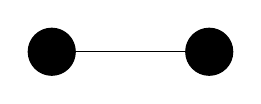
\begin{tikzpicture}
	 \def \radius {1cm}
	 \def \margin {8}
	 \def \n {2}
	 \foreach \s in {1,...,\n}
	  \node[draw, circle] (\s) at ({360/\n * (\s - 1)}:\radius) {};
	 \foreach \s in {1,...,\n}
	  \foreach \t in {\s,...,\n}
	   \draw (\t) -- (\s);
	\end{tikzpicture}
\end{minipage}
\begin{minipage}{.2\textwidth}
	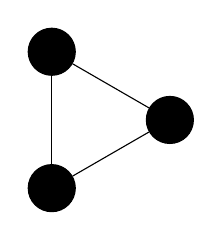
\begin{tikzpicture}
	 \def \radius {1cm}
	 \def \margin {8}
	 \def \n {3}
	 \foreach \s in {1,...,\n}
	  \node[draw, circle] (\s) at ({360/\n * (\s - 1)}:\radius) {};
	 \foreach \s in {1,...,\n}
	  \foreach \t in {\s,...,\n}
	   \draw (\t) -- (\s);
	\end{tikzpicture}
\end{minipage}
\begin{minipage}{.2\textwidth}
	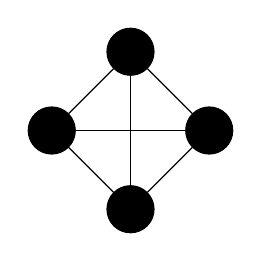
\begin{tikzpicture}
	 \def \radius {1cm}
	 \def \margin {8}
	 \def \n {4}
	 \foreach \s in {1,...,\n}
	  \node[draw, circle] (\s) at ({360/\n * (\s - 1)}:\radius) {};
	 \foreach \s in {1,...,\n}
	  \foreach \t in {\s,...,\n}
	   \draw (\t) -- (\s);
	\end{tikzpicture}
\end{minipage}
\begin{minipage}{.2\textwidth}
	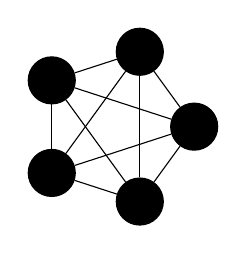
\begin{tikzpicture}
	 \def \radius {1cm}
	 \def \margin {8}
	 \def \n {5}
	 \foreach \s in {1,...,\n}
	  \node[draw, circle] (\s) at ({360/\n * (\s - 1)}:\radius) {};
	 \foreach \s in {1,...,\n}
	  \foreach \t in {\s,...,\n}
	   \draw (\t) -- (\s);
	\end{tikzpicture}
\end{minipage}
\begin{minipage}{.2\textwidth}
	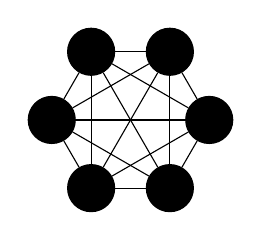
\begin{tikzpicture}
	 \def \radius {1cm}
	 \def \margin {8}
	 \def \n {6}
	 \foreach \s in {1,...,\n}
	  \node[draw, circle] (\s) at ({360/\n * (\s - 1)}:\radius) {};
	 \foreach \s in {1,...,\n}
	  \foreach \t in {\s,...,\n}
	   \draw (\t) -- (\s);
	\end{tikzpicture}
\end{minipage}
\end{exmp}

\begin{defn}
Un graphe ${\Gamma}'=(U,F)$ est un sous-graphe de $\Gamma=(V,E)$ si $ U \subseteq V$ et $F \subseteq E$. On notera $ {\Gamma}' \leq \Gamma$.
\end{defn}

\begin{exmp}
$ K_{m} \leq K_{n}$ si $ m \leq n$.
\end{exmp}

\begin{exo}
Montrer que $K_{m}$ possède $ q=\frac{1}{2}n(n-1)$ arêtes.
\end{exo}

%----------------------------------------------------

\subsection{Chemins dans les graphes}

\begin{defn}
Soit $\Gamma = (V,E)$ et $v,w \in V$. Un chemin de v à w de longueur n est une séquence alternée de $(n+1)$ sommets $v_{0},v_{1},\ldots,v_{n}$ et de n arêtes $e_{1},e_{2},\ldots,e_{n}$ de la forme $$ (v_{0},e_{1},v_{1},e_{2},\ldots,e_{n},v_{n})$$ dans laquelle chaque $e_{i}$ est incident à $v_{i-1}$ et $v_{i}$ pour $1 \leq i \leq n$ et $ e_{i} \neq e_{j} , \forall i \neq j \in 1,\ldots,n$ 

Un chemin est simple si aucun sommet ne se répète sauf peut-être $v_{0}$ et $v_{n}$. 

Dans un graphe simple on notera juste la suite des sommets lorsque l'on décrit un chemin. 

\end{defn}

\begin{defn}
Un graphe $\Gamma = (V,E)$ est connexe si $\forall x,y \in V : \exists $ un chemin de x à y. 

La composante connexe de $\Gamma$ contenant x est le sous-graphe ${\Gamma}'$ de $\Gamma$ dont les sommets et les arêtes sont contenus dans un chemin de $\Gamma$ démarrant en x. 
\end{defn}

\begin{defn}
Soit $\Gamma = (V,E)$ et $v \in V$.

Un cycle est un chemin de v à v.

Un cycle simple est un cycle de v à v dans lequel aucun sommet n'est répété (mis à part le départ et l'arrivée).
\end{defn}

\newpage

%----------------------------------------------------

\subsection{Arbres}

\subsubsection{Définitions}

\begin{defn}
Un arbre est un graphe simple connexe qui ne contient aucun cycle.
\end{defn}

\begin{defn}
Dans un arbre, les sommets de degré 1 sont appellés les feuilles.
\end{defn}

\begin{exmp}

\end{exmp}

\newcommand{\twochildren}{child{node{\null}} child{node{\null}}} 

\begin{figure}[!h]
\centering
	\begin{tikzpicture}[style=thick,rotate=-90,scale=0.8] 
	\tikzstyle{every node}=[circle,inner sep=2pt,draw] 
	\tikzstyle{level 1}=[sibling distance=20mm]
	\tikzstyle{level 2}=[sibling distance=10mm] 
	\tikzstyle{level 3}=[sibling distance=5mm] 
	\node{\null}[grow'=right] 
	child{node{\null} 
	child{node{\null}\twochildren} 
	child{node{\null}\twochildren} }
	child{node{\null} 
	child{node{\null}\twochildren} 
	child{node{\null}\twochildren} } 
	child{node{\null} 
	child{node{\null}\twochildren}
	child{node{\null}\twochildren} }; 
	\end{tikzpicture} 
\end{figure}

\begin{prop}
Si T est un arbre avec $p\geq2$ sommets, alors T contient au moins 2 feuilles.
\end{prop}

\begin{demo}
T a p sommets. Tous les chemins sont de longueur inférieure ou égale à p. Considérons un chemin $v_{0},v_{1},\ldots,v_{r}$ pour $v_{i} \in V$, $i=0,\ldots,r$ de longueur maximale. Alors, $v_{0}$ et $v_{r}$ sont de degré 1.
\end{demo}

\begin{thrm}[\textcolor{red}{ATTENTION! Ce théorème et sa démonstration font partie de ceux à connaitre par coeur à l'examen! (pour l'année 2015-2016)}]
Soit T un graphe simple à p sommets. Alors les 3 assertions suivantes sont équivalentes:
	\begin{enumerate}[i]
		\item T est un arbre.
		\item T a $(p-1)$ arêtes et aucun cycle.
		\item T a $(p-1)$ arêtes et est connexe.
	\end{enumerate}
\end{thrm}

\begin{demo}

$\mathbf{(i) \Rightarrow (ii)}$\textbf{: Montrer qu'un arbre à p sommets a (p-1) arêtes.}

	Par récurrence:
		\begin{enumerate}
			\item p = 1 OK 
			\item Supposons que ce soit vrai pour tout arbre à $ k \geq 1$ sommets et montrons le pour un arbre à (k+1) sommets. Soit T un tel arbre, il a au moins 2 feuilles. Enlevons une de ces feuilles ainsi que l'arête incidente. On obtient un arbre ${T}'$ à k sommets. Par l’hypothèse de récurrence: ${T}'$ a (k-1) arêtes, donc T a k arêtes.
		\end{enumerate} 

\hspace{-0.5cm}$\mathbf{(ii) \Rightarrow (iii)}$\textbf{: Supposons (ii) et T ne soit pas connexe.}

	Notons $T_{1}, T_{2},\ldots,T_{t}$ les composantes connexes de T avec $t \geq 2$. Chaque $T_{i}$ est un arbre, pour $1 \leq i \leq t$ (car pas de cycle). Soit $p_{i}$ le nombre de sommets de $T_{i}$, alors chaque $T_{i}$ a $(p_{i}-1)$ arêtes.

	\begin{minipage}{.5\textwidth}
		\[\sum_{i=1}^{t} p_{i} = p$$ et $$p-1 = \sum_{i=1}^{t} (p_{i}-1) = p - t \]
	\end{minipage}
	\begin{minipage}{.5\textwidth}
		donc $\Rightarrow t = 1 $
	\end{minipage}

\hspace{-0.5cm}$\mathbf{(iii) \Rightarrow (i)}$\textbf{: Supposons que T ne soit pas un arbre.}

	Alors, T contient un cycle C. Enlevons une arête de C. On obtient le sous-graphe ${T}'$ de T qui est toujours connexe. Si ${T}'$ contient un cycle, alors on itère le processus. Sinon, ${T}'$ est un arbre à p sommets qui a strictement moins que (p-1) arêtes.
		
\end{demo}

% COURS 2

\subsubsection{Arbres couvrants et arbres à poids}

\begin{defn}
Un arbre couvrant dans un graphe $\Gamma$ est un arbre qui est un sous-graphe de $\Gamma$ et qui contient tous les sommets de $\Gamma$.
\end{defn}

Dans certains problèmes, certaines arêtes sont plus importantes que d'autres. En théorie des graphes, on modélise cela en assignant une valeur à chaque arête. 

\begin{defn}
Un arbre à poids est un couple $(\Gamma,w)$ où $\Gamma$ est un arbre w est une fonction $w: E \rightarrow \mathbb{R}^{+}$. Le nombre w(e) est appelé le poids de l'arête e.
\end{defn}

\begin{exmp}

\end{exmp}



\begin{figure}[htb]
\centering
	\begin{tikzpicture}[scale=0.4]	
		\SetUpEdge[lw = 1.5pt,color = black,labelcolor = white]
		\GraphInit[vstyle=Normal] 
		\SetGraphUnit{3}
		\tikzset{VertexStyle/.append  style={fill}}
		\Vertex{P}
		\NOEA(P){B}  \SOEA(P){M} \NOEA(B){D}
		\SOEA(B){C}  \SOEA(C){L}
		\tikzset{EdgeStyle/.style={-}}
		\Edge[label=$3$](C)(B)
		\Edge[label=$10$](D)(B)
		\Edge[label=$10$](L)(M)
		\Edge[label=$10$](B)(P)
		\Edge[label=$4$](P)(M)
		\Edge[label=$9$](C)(M)
		\Edge[label=$4$](C)(L)
		\Edge[label=$5$](C)(D)
		\Edge[label=$10$](B)(M)
		\Edge[label=$11$](L)(D)
	\end{tikzpicture}  

\end{figure}

%----------------------------------------------------
\newpage

\subsection{Isomorphisme}

\begin{defn}
Deux graphes $\Gamma_{1} = (V_{1},E_{1},\gamma_{1})$ et $\Gamma_{2} = (V_{2},E_{2},\gamma_{2})$ sont isomorphes s'il existe une bijection $f: V_{1} \rightarrow V_{2}$ et une bijection $g: E_{1} \rightarrow E_{2}$ telles que $\forall e \in E_{1}:$ e est incident à v,w $\in V_{1}$ ssi g(e) est incident à f(v),f(w) $\in V_{2}$. Le couple (f,g) est appelé un isomorphisme de graphe et on note $\Gamma_{1} \cong \Gamma_{2}$.
\end{defn}

Deux graphes isomorphes ont les mêmes propriétés.

\begin{exmp}

\end{exmp}

\begin{figure}[!htb,scale=0.8]
  \centering

  \begin{minipage}{.2\textwidth}

     \begin{tikzpicture}[>=stealth',shorten >=1pt,auto,node distance=1.5cm,thick,main node/.style={circle,draw,font=\sffamily\large\bfseries}]

    \node[main node] (a) {$a$};
    \node[main node] (b) [right of=a] {$b$};
    \node[main node] (c) [below of=a] {$c$};
    \node[main node] (d) [right of=c] {$d$};


    \path[every node/.style={font=\sffamily\small}]
    (a) edge node [right] {} (b)
       edge node [below] {} (c)
       edge node [right] {} (d)
    (c) edge node [right] {} (b)
    (d) edge node [above] {} (b)
       edge node [left] {} (c);

    \end{tikzpicture}

  \end{minipage}
  \begin{minipage}{.2\textwidth}
    \begin{tikzpicture}[>=stealth',shorten >=1pt,auto,node distance=1.5cm,thick,main node/.style={circle,draw,font=\sffamily\large\bfseries}]

      \node[main node] (d) {${d}'$};
      \node[main node] (a) [above of=d] {${a}'$};
      \node[main node] (c) [below left of=d] {${c}'$};
      \node[main node] (b) [below right of=d] {${b}'$};


      \path[every node/.style={font=\sffamily\small}]
      (a) edge node [right] {} (b)
         edge node [below] {} (c)
         edge node [right] {} (d)
      (c) edge node [right] {} (b)
      (d) edge node [above] {} (b)
         edge node [left] {} (c);

    \end{tikzpicture}
  \end{minipage}

  \caption{ Deux graphes isomorphes }
\end{figure}

%----------------------------------------------------

\subsection{Graphes hamiltoniens}

Hamilton propose le problème suivant: Considérons le graphe du dodécaèdre. Est-il possible, en partant d'un des vingts sommets et en suivant les arêtes du graphe, de visiter tous les sommets une et une seule fois et de revenir au sommet de départ? 

L'exemple suivant montre un chemin qui réponds à ce problème. 

\begin{exmp}

\end{exmp}

\begin{figure}[htb]
\centering
	
	\begin{minipage}{.4\textwidth}
	\hspace{-1.5cm}
	    \begin{tikzpicture}[scale=0.8]
			\grDodecahedral[form=2] 
		\end{tikzpicture}

	\end{minipage}
	\begin{minipage}{.4\textwidth}
	\hspace{1.5cm}
		\begin{tikzpicture}[scale=0.8]
			\grDodecahedral[form=2]
			\Edges[local,color=red,lw=4pt](a3,b3,c2,b2,c1,b1,c0,b0,c4,d4,d0,d1,d2,d3,c3,b4,a4,a0,a1,a2,a3)
		\end{tikzpicture}
	\end{minipage}

\caption{ Graphe hamiltonien et cycle hamiltonien}
\end{figure}

\newpage

\begin{defn}
Un cycle hamiltonien dans un graphe $\Gamma$ est un cycle simple contenant tous les sommets de $\Gamma$. 
\end{defn}

Pour donner un exemple de graphe non-hamiltonien on introduit la notion de graphe biparti. 

\begin{defn}
Un graphe $\Gamma = (V,E)$ est biparti si on peu écrire $V=B \cup W$ avec $B \cap W = \varnothing $ et toute arête de $\Gamma$ joint un sommet dans B à un sommet dans W.
\end{defn}

\begin{exmp}

\end{exmp}

\begin{figure}[!h]
\centering
	\begin{tikzpicture}

	\tikzstyle{every node}=[draw,minimum size=10pt,inner sep=2pt]
	\tikzstyle{every label}=[position=above]
	\tikzstyle{frame_blue} = [line width=2pt, draw=blue, inner sep=0.2em, minimum width=1cm,minimum height=2cm]
	\tikzstyle{frame_red} = [line width=2pt, draw=red, inner sep=0.2em, minimum width=1cm,minimum height=2cm]

	\node[circle,fill=red] (r1) at (1,-0.5) { };
	\node[circle,fill=red] (r2) at (1,-1.5) { };
	\node[circle,fill=red] (r3) at (1,0.5) { };
	\node[circle,fill=red] (r4) at (1,1.5) { };
	\node[circle,fill=blue] (b1) at (3,0.5) { };
	\node[circle,fill=blue] (b2) at (3,-0.5) { };

	\draw  (r4) edge (b1);
	\draw  (b1) edge (r3);
	\draw  (r3) edge (b2);
	\draw  (b2) edge (r1);
	\draw  (r2) edge (b1);

	\node[frame_red,fit=(r1)(r2)(r3)(r4)]{ };
	\node[frame_blue,fit=(b1)(b2)]{ };

	\end{tikzpicture}
\caption{B en rouge, W en bleu}
\end{figure}

\begin{lemme}
Si $\Gamma$ est biparti, alors $\Gamma$ ne contient pas de cycle simple de longueur impaire.
\end{lemme}

\begin{thrm}
Un graphe biparti avec un nombre impaire de sommets n'est pas hamiltonien.
\end{thrm}

\begin{demo}
Pour être hamiltonien, il doit admettre un cycle simple passant par tous ses sommets, donc de longueur impaire. Ce n'est pas possible à cause du Lemme précédent.
\end{demo}

\begin{exmp}

\end{exmp}

\begin{figure}[!h]
\centering
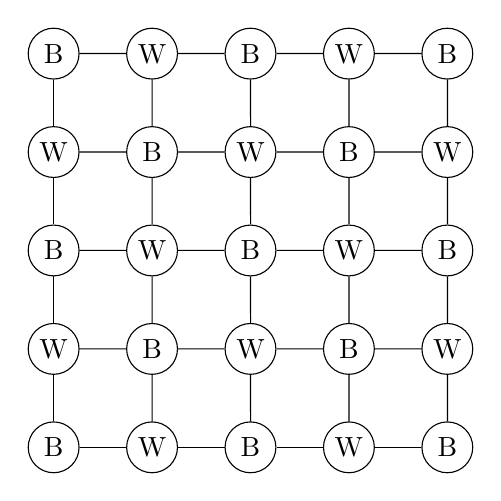
\begin{tikzpicture}[scale = 0.5,xscale=2.5,yscale=2.5]

\tikzstyle{every node}=[draw,circle,fill=black,minimum size=5pt,inner sep=0pt,text width=6mm,align=center]

\node (a00) at (0,0) [shape= circle, draw, fill = white] {B};
\node (a10) at (1,0) [shape= circle, draw, fill = white] {W};
\node (a20) at (2,0) [shape= circle, draw, fill = white] {B};
\node (a30) at (3,0) [shape= circle, draw, fill = white] {W};
\node (a40) at (4,0) [shape= circle, draw, fill = white] {B};

\node (a01) at (0,1) [shape= circle, draw, fill = white] {W};
\node (a11) at (1,1) [shape= circle, draw, fill = white] {B};
\node (a21) at (2,1) [shape= circle, draw, fill = white] {W};
\node (a31) at (3,1) [shape= circle, draw, fill = white] {B};
\node (a41) at (4,1) [shape= circle, draw, fill = white] {W};

\node (a02) at (0,2) [shape= circle, draw, fill = white] {B};
\node (a12) at (1,2) [shape= circle, draw, fill = white] {W};
\node (a22) at (2,2) [shape= circle, draw, fill = white] {B};
\node (a32) at (3,2) [shape= circle, draw, fill = white] {W};
\node (a42) at (4,2) [shape= circle, draw, fill = white] {B};

\node (a03) at (0,3) [shape= circle, draw, fill = white] {W};
\node (a13) at (1,3) [shape= circle, draw, fill = white] {B};
\node (a23) at (2,3) [shape= circle, draw, fill = white] {W};
\node (a33) at (3,3) [shape= circle, draw, fill = white] {B};
\node (a43) at (4,3) [shape= circle, draw, fill = white] {W};

\node (a04) at (0,4) [shape= circle, draw, fill = white] {B};
\node (a14) at (1,4) [shape= circle, draw, fill = white] {W};
\node (a24) at (2,4) [shape= circle, draw, fill = white] {B};
\node (a34) at (3,4) [shape= circle, draw, fill = white] {W};
\node (a44) at (4,4) [shape= circle, draw, fill = white] {B};

\draw (a00) -- (a01) -- (a02) -- (a03) -- (a04);
\draw (a10) -- (a11) -- (a12) -- (a13) -- (a14);
\draw (a20) -- (a21) -- (a22) -- (a23) -- (a24);
\draw (a30) -- (a31) -- (a32) -- (a33) -- (a34);
\draw (a40) -- (a41) -- (a42) -- (a43) -- (a44);

\draw (a00) -- (a10) -- (a20) -- (a30) -- (a40);
\draw (a01) -- (a11) -- (a21) -- (a31) -- (a41);
\draw (a02) -- (a12) -- (a22) -- (a32) -- (a42);
\draw (a03) -- (a13) -- (a23) -- (a33) -- (a43);
\draw (a04) -- (a14) -- (a24) -- (a34) -- (a44);
\end{tikzpicture}
\caption{Graphe biparti mais non hamiltonien.}
\end{figure}

% COURS 3

\newpage

\begin{thrm}[Dirac 1950]
Soit $\Gamma = (V,E)$ un graphe simple avec $p \geq 3$ sommets. Si $\forall v \in V: deg(v) \geq \frac{1}{2}p$, alors $\Gamma$ est Hamiltonien.
\end{thrm}

\begin{demo}
$\Gamma$ est connexe. Soit C = $(v_{0},v_{1},\ldots,v_{k})$ un plus long chemin simple dans $\Gamma$ avec $v_{0} \neq v_{k}, k < p$.

$ deg(v_{0}) \geq \frac{p}{2}$, tous les sommets adjacents à $v_{0}$ sont dans $\{v_{1},\ldots,v_{k}\}$

$ deg(v_{k}) \geq \frac{p}{2}$, tous les sommets adjacents à $v_{k}$ sont dans $\{v_{0},\ldots,v_{k-1}\}$

Comme $k < q$, il doit exister $i \in \{0,\ldots,k-1\}$ tel que $\{v_{i},v_{k}\} \in E$ et $\{v_{0},v_{i+1}\} \in E$. 

On obtient un cycle $\widetilde{C} = (v_{0},v_{1},\ldots,v_{i},v_{k},v_{k-1},\ldots,v_{i+1},v_{0})$ 

\begin{figure}[htb]
	\centering
	\begin{tikzpicture}[mydot/.style={fill,circle,inner sep=2pt},]

		\node[mydot,label={$v_{0}$}] (v0) {};
		\node[mydot,below right=of v0] (v1) {};
		\node[mydot,above right=of v1] (v2) {};
		\node[mydot,below right=of v2,label={$v_{i}$}] (v3) {};
		\node[mydot,above right=of v3,label={$v_{i+1}$}] (v4) {};
		\node[mydot,below right=of v4] (v5) {};
		\node[mydot,above right=of v5] (v6) {};
		\node[mydot,right=of v6] (v7) {};
		\node[mydot,above right=of v7] (v8) {};
		\node[mydot,above right=of v8,label={$v_{k}$}] (v9) {};
		\begin{pgfonlayer}{background}
		\Twocolor{(v0)}{(v1)}{red}{green}
		\Twocolor{(v1)}{(v2)}{red}{green}
		\Twocolor{(v2)}{(v3)}{red}{green}
		\Twocolor{(v4)}{(v5)}{green}{red}
		\Twocolor{(v5)}{(v6)}{green}{red}
		\Twocolor{(v6)}{(v7)}{green}{red}
		\Twocolor{(v7)}{(v8)}{green}{red}
		\Twocolor{(v8)}{(v9)}{green}{red}
		\end{pgfonlayer}
		\draw[red,line width=1pt] 
			(v3) -- (v4);
		\draw[green,line width=1pt] 
			(v0) to[out=45,in=135] (v4)
			(v3) to[out=-45,in=-20,looseness=1] (v9);
	\end{tikzpicture}

	\caption{Les 2 chemins, C en rouge, $\widetilde{C}$ en vert.}
\end{figure}

On note que $\widetilde{C}$ est un cycle Hamiltonien.

Supposons:

$\exists  y \in \widetilde{C} \Rightarrow$ On peut supposer que $\{ v_{j},y\} \in E$ pour $j=\{0,\ldots,k\}$.

$\Rightarrow$ On construit un chemin $\overline{C} = (y, v_{j},v_{j-1},\ldots v_{0},v_{i+1},\ldots,v_{k},v_{i},v_{i-1},\ldots,v_{j-1})$. $\overline{C}$ est un chemin plus long que C. 

\begin{figure}[H]
	\centering
	\begin{tikzpicture}[mydot/.style={fill,circle,inner sep=2pt},]

		\node[mydot] (v0) {};
		\node[mydot,below right=of v0] (v1) {};
		\node[mydot,above right=of v1,label={$v_{j}$}] (v2) {};

		\node[mydot,below=of v2,label={[yshift=-0.6cm]$y$}] (y) {};
		\node[mydot,above left= 0.5cm of v3,label={$v_{j+1}$}] (vj1) {};

		\node[mydot,below right=of v2] (v3) {};
		\node[mydot,above right=of v3] (v4) {};
		\node[mydot,below right=of v4] (v5) {};
		\node[mydot,above right=of v5] (v6) {};
		\node[mydot,right=of v6] (v7) {};
		\node[mydot,above right=of v7] (v8) {};
		\node[mydot,above right=of v8] (v9) {};
		\draw[green,line width=1pt] 
			(v0) -- (v1) -- (v2);
		\draw[green, line width=1pt]
			(v4) -- (v5) -- (v6) -- (v7) -- (v8) -- (v9);
		\draw[green, line width=1pt]
			(v3) -- (vj1);
		\draw[green, line width=1pt]
			(v2) -- (y);
		\draw[green,line width=1pt] 
			(v0) to[out=45,in=135] (v4)
			(v3) to[out=-45,in=-20,looseness=1] (v9);
	\end{tikzpicture}

	\caption{Chemin $\overline{C}$}
\end{figure}

\end{demo}

\newpage

\textbf{Illustration: Code de Gray}

Un code de Gray d'ordre n est un arrangement cyclique de $2^{n}$ mots binaires de longueur n tels que 2 mots adjacents ne diffèrent qu'en une seule position.

\begin{exmp}
Le code de Grey ci-dessous provient d'un cycle hamiltonien sur le graphe du cube:
\end{exmp}

\begin{figure}[!tbph]
  \centering
  \begin{minipage}[b]{0.4\textwidth}
    \def\sector#1#2#3#4#5{%
\fill[#5] (#1) -- (#3:#2) arc (#3:#4:#2) -- cycle;
}

% Define colors for bits 1 and 0
\colorlet{color1}{red!50!white}
\colorlet{color0}{white}

\begin{figure}[!h]
\centering

  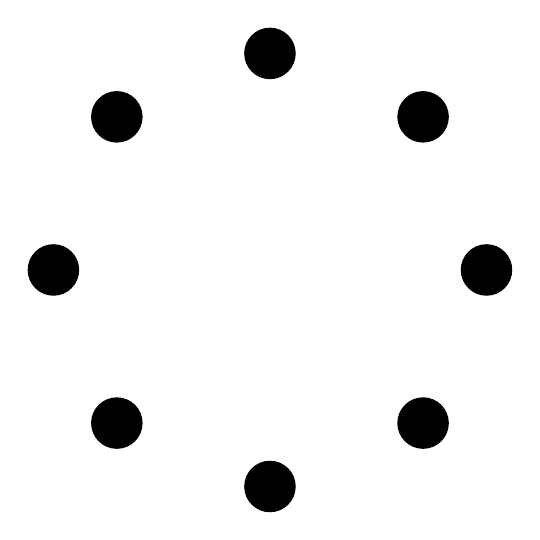
\begin{tikzpicture}[scale=0.5]
      \foreach \code [count=\i from=1] in {110,010,000,001,011,111,101,100} {
        \node at (\i*45:5.5) {\code}; % Label each code
        % Draw sectors from outside to inside
        \foreach \r in  {5,3,1} {
           \StrRight{\code}{1}[\bit]         % Get the rightmost bit
           \StrGobbleRight{\code}{1}[\code]  % Get the remaining left bits
           \xdef\code{\code}  % Set them for the next iteration
           \sector{0,0}{\r}{45*\i}{45*\i-45}{color\bit, draw=black, thick}
         }
      }
  \end{tikzpicture}
  
\end{figure}
  \end{minipage}
  \hfill
  \begin{minipage}[b]{0.4\textwidth}
    
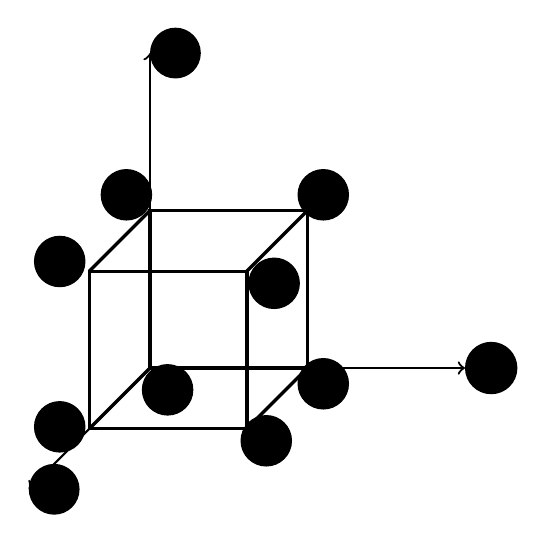
\begin{tikzpicture}
    [cube/.style={very thick,black},
      grid/.style={very thin,gray},
      axis/.style={->,black,thick}]
      
  %draw the axes
  \draw[axis] (0,0,0) -- (4,0,0) node[anchor=west]{$y$};
  \draw[axis] (0,0,0) -- (0,4,0) node[anchor=west]{$z$};
  \draw[axis] (0,0,0) -- (0,0,4) node[anchor=west]{$x$};

  %draw the top and bottom of the cube
  \draw[cube] (0,0,0) -- (0,2,0) -- (2,2,0) -- (2,0,0) -- cycle;
  \draw[cube] (0,0,2) -- (0,2,2) -- (2,2,2) -- (2,0,2) -- cycle;
  
  %draw the edges of the cube
  \draw[cube] (0,0,0) -- (0,0,2);
  \draw[cube] (0,2,0) -- (0,2,2);
  \draw[cube] (2,0,0) -- (2,0,2);
  \draw[cube] (2,2,0) -- (2,2,2);

  %labels
  \node (O) at (0.3,-0.2,0.2) {$000$};
  \node (A) at (-0.3,2.2,0) {$001$};
  \node (B) at (-0.3,2.2,2.2) {$101$};
  \node (C) at (-0.3,0.1,2.2) {$100$};
  \node (D) at (2.2,2.2,0) {$011$};
  \node (E) at (2.2,-0.2,0) {$010$};
  \node (F) at (2.5,2,2.4) {$111$};
  \node (G) at (2.4,0,2.4) {$110$};

\end{tikzpicture}
  \end{minipage}
\end{figure}

Un code de Gray d'ordre (n+1) se construit à partir d'un code de Gray d'ordre n comme suit:

\begin{enumerate}
	\item On écrit le code de Gray donné d'ordre n en ajoutant à la fin de chaque mot un zéro.
	\item On le fait suivre par le même code de Gray parcouru dans l'autre sens et en ajoutant à la fin de chaque mot un 1.
\end{enumerate}

%----------------------------------------------------

\subsection{Graphes Eulériens}

\begin{defn}
Un cycle Eulérien dans un graphe $\Gamma$ est un cycle qui contient toutes les arêtes de $\Gamma$.
Un graphe est Eulérien s'il contient un cycle Eulérien.
\end{defn}

\begin{prop}
Si un graphe est Eulérien, alors tous ses sommets sont de degré pair.
\end{prop}

\begin{lemme}
Soit $\Gamma$ un graphe dans lequel chaque sommet est de degré pair, alors l'ensemble E se partitionne en une union de cycles (arête-)disjointe.
\end{lemme}

\begin{exmp}

\end{exmp}
\begin{figure}[!h]
\centering

	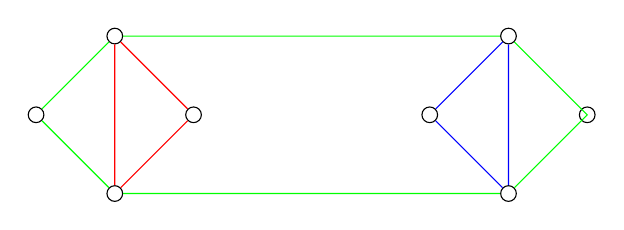
\begin{tikzpicture}
	\tikzstyle{every node}=[circle,inner sep=2pt,draw] 
	\node (v7) at (-1,0) {};
	\node (v3) at (1,0) {};
	\node (v2) at (0,1) {};
	\node (v1) at (0,-1) {};
	\node (v6) at (4,0) {};

	\node at (6,0) {};
	\node (v5) at (5,1) {};
	\node (v4) at (5,-1) {};
	\draw[red] (v1) -- (v2) -- (v3) -- (v1);
	\draw[blue] (v4) -- (v5) -- (v6) -- (v4);
	\draw[green] (v1) -- (v7) -- (v2) -- (v5) -- (6,0) -- (v4) -- (v1);
	\end{tikzpicture}
	
\end{figure}

\newpage

\begin{demo}
Par récurrence, sur le nombre d'arêtes
	\begin{enumerate}
		\item Le lemme est vrai pour $q=2$.
		\item Supposons qu'il soit vrai pour tout graphe à $q \leq k$ arêtes et montrons-le pour un graphe à (k+1) arêtes.
		\item Soit $v_{0}$ un sommet de $\Gamma$. On démarre un chemin en $v_{0}$ et on le suit jusqu'à ce qu'un sommet soit répété 2 fois. On le note $v_{j}$ et C le cycle de $v_{j}$ à $v_{j}$.
		\item Soit ${\Gamma}'$ le sous-graphe de $\Gamma$, obtenu par $V={V}'$ et ${E}'=E \setminus C$. ${\Gamma}'$ a $\#{E}' \leq k$ arêtes. Par hypothèse de récurrence, les arêtes de ${\Gamma}'$ se partitionnent en une union arête-disjointe de cycles $C_{1} \cup C_{2} \cup \ldots \cup C_{n}$.
		\item Donc, $C_{1} \cup C_{2} \cup \ldots \cup C_{n}$ est une partition arête-disjointe des arêtes de $\Gamma$.
	\end{enumerate}
\end{demo}

\begin{thrm}[\textcolor{red}{ATTENTION! Ce théorème et sa démonstration font partie de ceux à connaitre par coeur à l'examen! (pour l'année 2015-2016)}]
Soit $\Gamma$ un graphe connexe. Alors, $\Gamma$ est eulérien si et seulement si chaque sommet a un degré pair.
\end{thrm}

\begin{demo}
$\Rightarrow$ OK par proposition précédente.

\hspace{-0.60cm}$\Leftarrow$ Par le Lemme: E se partitionne en une union (arête-)disjointe de cycles $C_{1} \cup C_{2} \cup \ldots \cup C_{n}$.
	\begin{enumerate}
		\item Si n=1, c'est bon.
		\item Si $n>1$, comme $\Gamma$ est connexe, $\exists$ une arête incidente à un $v \in C_{1}$ et un $w \notin C_{1}$. Cette arête est dans $C_{j}$ pour un $j=2,\ldots,n$ (car on a une partition de E). On attache ce cycle en v. S'il reste des cycles dans la partition, on itère ce procédé jusqu'à avoir utilisé tous les cycles.
	\end{enumerate}
\end{demo}
%----------------------------------------------------

\subsection{Application: le problème du voyageur de commerce (TSP)}

\subsubsection{Énoncé du problème}

Énoncé: Un vendeur de livres démarre de chez lui et doit visiter un certain nombre de librairies avant de rentrer chez lui. Comment doit-il choisir sa route pour minimiser la distance parcourue?  

Objet mathématique: Un graphe valué (à chaque arête est associé un nombre appelé poids) où les sommets représentent les librairies et les arêtes représentent les routes.

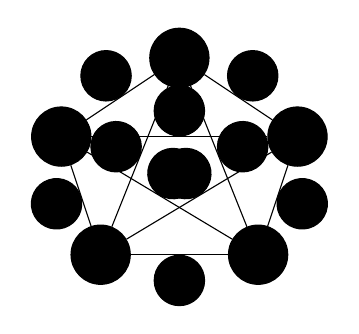
\begin{tikzpicture}


\node[circle,inner sep=2pt,draw]  (v2) at (0,0) {};
\node[circle,inner sep=2pt,draw]  (v1) at (-1.5,-1) {};
\node[circle,inner sep=2pt,draw]  (v3) at (1.5,-1) {};
\node[circle,inner sep=2pt,draw]  (v5) at (-1,-2.5) {};
\node[circle,inner sep=2pt,draw]  (v4) at (1,-2.5) {};

\draw  (v1) -- (v2) node [above,midway,sloped] {3} ;
\draw  (v2) -- (v3) node [above,midway,sloped] {7};
\draw  (v3) -- (v4) node [below,midway,sloped] {4};
\draw  (v4) -- (v5) node [below,midway,sloped] {4};
\draw  (v5) -- (v1) node [below,midway,sloped] {7};

\draw  (v5) -- (v2) node [above,midway,sloped] {6};
\draw  (v2) -- (v4) node [above,midway,sloped] {6};
\draw  (v4) -- (v1) node [above,midway,sloped] {7};
\draw  (v1) -- (v3) node [above,midway,sloped] {8};
\draw  (v3) -- (v5) node [above,midway,sloped] {3};


\end{tikzpicture}

Objectif: Trouver un cycle hamiltonien de poids minimal.

Remarque: Un graphe complet $K_{n}$ à n sommets possède $\frac{1}{2}(n-1)!$ cycles hamiltoniens différents. Par exemple, pour $n=10 \Rightarrow$ 181440 cycles. On ne connait pas encore d'algorithme efficace qui donne une solution au problème.

\newpage

\subsubsection{Arbres couvrant minimum}

\begin{defn}
Un arbre couvrant dans un graphe $\Gamma$ est un arbre qui est un sous-graphe de $\Gamma$ et qui contient tous les sommets de $\Gamma$.
\end{defn}

Il existe un algorithme qui donne des arbres couvrants de poids minimum dans un graphe valué.

Algorithme de Kurskal:
\begin{enumerate}[i]
	\item Choisir une arêtes de plus petit poids.
	\item Choisir parmi les arêtes restantes une arête de plus petit poids dont l'inclusion ne crée pas un cycle.
	\item Continuer jusqu'à obtenir un arbre couvrant.
\end{enumerate}

\begin{exmp}

\end{exmp}
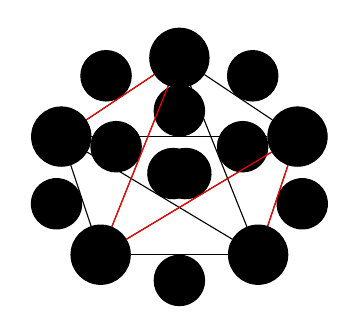
\begin{tikzpicture}


\node[circle,inner sep=2pt,draw]  (v2) at (0,0) {};
\node[circle,inner sep=2pt,draw]  (v1) at (-1.5,-1) {};
\node[circle,inner sep=2pt,draw]  (v3) at (1.5,-1) {};
\node[circle,inner sep=2pt,draw]  (v5) at (-1,-2.5) {};
\node[circle,inner sep=2pt,draw]  (v4) at (1,-2.5) {};

\draw  (v1) -- (v2) node [above,midway,sloped] {3} ;
\draw  (v2) -- (v3) node [above,midway,sloped] {7};
\draw  (v3) -- (v4) node [below,midway,sloped] {4};
\draw  (v4) -- (v5) node [below,midway,sloped] {4};
\draw  (v5) -- (v1) node [below,midway,sloped] {7};

\draw  (v5) -- (v2) node [above,midway,sloped] {6};
\draw  (v2) -- (v4) node [above,midway,sloped] {6};
\draw  (v4) -- (v1) node [above,midway,sloped] {7};
\draw  (v1) -- (v3) node [above,midway,sloped] {8};
\draw  (v3) -- (v5) node [above,midway,sloped] {3};

\draw[red] (v1) -- (v2) -- (v5) -- (v3) -- (v4);
\end{tikzpicture}

Remarque: Si C est un cycles hamiltonien dans un graphe $\Gamma$, alors $\forall e \in E$ arête de C: $ C \setminus\{e\}$ est un arbre couvrant.

$\Rightarrow$ (Solution de TSP) $\geq$ (longueur minimum d'un arbre couvrant)

Mieux: Soit v un sommet de $\Gamma$. Tout cycle hamiltonien contient 2 arêtes incidentes à v. Le reste du chemin est un arbre couvrant de $\Gamma \setminus\{v\}$.

$\Rightarrow$ (Solution de TSP) $\geq (\sum$ des longueurs des 2 plus courtes arêtes incidentes à v) + (longueur minimum d'un arbre couvrant de $\Gamma \setminus\{v\}$)

Remarque: Il existe une borne supérieure à TSP en utilisant des cycles eulériens. 

%----------------------------------------------------

\newpage

\subsection{Ordres partiels}

\textbf{ [ Ce dernier sous-chapitre est en désordre total, un truc plus structuré arrive bientôt. ] } 

\begin{defn}
Soit P un ensemble. Un ordre partiel sur P est une relation sur P, c'est à dire un ensemble de couples $(p_{1},p_{2}) \in P\times P$, noté $p{1} \leq p{2}$ tel que:
	\begin{enumerate}
		\item $p \leq p$ (réflexive)
		\item $(p \leq q$ et $q \leq p ) \Rightarrow p = q$ (anti-symétrique)
		\item $(p \leq q$ et $q \leq r ) \Rightarrow p \leq r$ (transitive)
	\end{enumerate}
On note $(P,\leq)$ un ensemble partiellement ordonné.
\end{defn}

Remarque: Soit $(P,\leq)$ un ensemble partiellement ordonné, alors on définit un ordre partiel $\geq$ par: $$x \geq y \Leftrightarrow y \leq x$$

\begin{defn}
Soit P un ensemble.
	\begin{enumerate}
		\item $(P,\leq)$ est dit totalement ordonné si $\forall p_{1},p_{2} \in P$, $p_{1} \leq p_{2}$ ou $p_{2} \leq p_{1}$
		\item Soit $(P,\leq)$ un ordre partiel: une chaîne C est un sous-ensemble de P qui est totalement ordonné.
	\end{enumerate}
\end{defn}

\begin{exmp}
$(\mathbb{N},\leq)$

\hspace{-0.55cm}$(\mathbb{N},\mid)$ où $a \mid b$ si $\exists c \in \mathbb{Z}$ tel que $a \cdot c = b$ $(a,b \in \mathbb{Z})$
\end{exmp}

% COURS 4

\textbf{Lien avec la théorie des graphes:} 

Une relation d'ordre partiel peut se représenter à l'aide d'un graphe dirigé, mais il est très compliqué. On le simplifie en laissant tomber toutes les relations qui s’obtiennent par transitivité et les lacets.

Par transitivité et anti-symétrie: on sait qu'il n'y a pas de cycles, on peut se passer des flèches et on note de bas en haut.

Ex: (\{1,2,3,4,5,6,10,12,15,20,30,60\}, |)

\begin{figure}[!htc]
\centering

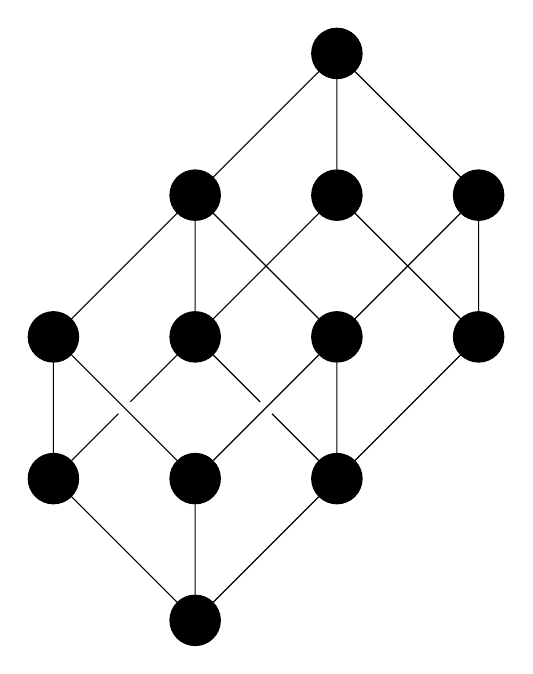
\begin{tikzpicture}[scale=0.9]
  \node (newmax) at (2,6) {$60$};
  \node (newb) at (2,4) {$20$};
  \node (newc) at (4,4) {$12$};
  \node (newf) at (4,2) {$4$};

  \node (max) at (0,4) {$30$};
  \node (a) at (-2,2) {$15$};
  \node (b) at (0,2) {$10$};
  \node (c) at (2,2) {$6$};
  \node (d) at (-2,0) {$5$};
  \node (e) at (0,0) {$3$};
  \node (f) at (2,0) {$2$};
  \node (min) at (0,-2) {$1$};

  \draw (min) -- (d) -- (a) -- (max) -- (b) -- (f)
  (e) -- (min) -- (f) -- (c) -- (max)
  (d) -- (b)
  (newf) -- (newb) -- (newmax) -- (newc) -- (newf)
  (max) -- (newmax)
  (b) -- (newb)
  (c) -- (newc)
  (f) -- (newf);

  \draw[preaction={draw=white, -,line width=6pt}] (a) -- (e) -- (c);
\end{tikzpicture}
\caption{Diagramme de Hasse}
\end{figure}

\begin{defn}
Soit $(P,\leq)$ un ensemble partiellement ordonné. Une anti-chaîne est un sous-ensemble A de P tel que $\forall a_{1},a_{2} \in A: $ $ a_{1} \nleqslant a_{2} $ et $ a_{2} \nleqslant a_{1} $
\end{defn}

\begin{exmp}
(\{1,2,3,6,8\},|), A = \{2,3\} est une anti-chaîne.
\end{exmp}

\begin{thrm}[Dilworth]
Soit $(P,\leq)$ un ensemble fini partiellement ordonné. Alors il existe une anti-chaîne A et une partition Q de P par des chaînes telle que $\#Q = \#A$.
\end{thrm}

\textbf{Lien avec les graphes bipartis:}

\begin{thrm}
Soit $\Gamma = (V,E)$ un graphe simple. 
	\begin{enumerate}
		\item Un couplage M de $\Gamma$ est un sous-ensemble d'arêtes de $\Gamma$, 2 à 2 non adjacentes. Les sommets incidents aux arêtes de M sont dits couplés.
		\item Un transversal de $\Gamma$ est un sous-ensemble T de V tel que toute arêtes $\Gamma$ est incidente à au moins un sommet de T.
	\end{enumerate}
\end{thrm}

\begin{thrm}[König]
Soit $\Gamma = (B \vmodels W, E)$ un graphe biparti. La cardinalité maximale d'un couplage de $\Gamma$ est égale à la cardinalité minimum d'un transversal de $\Gamma$.
\end{thrm}

\begin{exmp}
<PAGE 23>
\end{exmp}

\begin{defn}
Soit $\Gamma = (B \vmodels W, E)$ un graphe biparti et M un couplage. Un chemin alterné est un chemin qui démarre en un sommet non-couplé de B et alterne une arrête de E|M puis une arrête dans M et ainsi de suite.
\end{defn}

\begin{exmp}
<PAGE 23>
\end{exmp}

\newpage

\begin{demo}
<PAGE NOTE 2 et 3>
\end{demo}
% COURS 5

\begin{demo}
On va montrer König $\Rightarrow$ Dilworth.

Soit $(P,\leq)$ un ordre partiel. On construit un graphe biparti $\Gamma = ( B \vmodels W, E)$ où B = $\{ (p,1) | p \in P \}$ et W = $\{ (p,2) | p \in P \}$ et $\{ (p,1) , (q,2) \} \in E \Leftrightarrow p \leq q$ et $ p \neq q$. 

Soit M un couplage de cardinalité maximale de $\Gamma$ et T un transversal de cardinalité minimale de $\Gamma$. Par König, $\#M = \#T$.

On définit $A \subseteq P$ par $A = \{ p \in P | (p,1) \in T$ et $(p,2) \nsubseteq T \}$ et $\#A \geq \#P - \#T$. 

On construit des chaînes comme suit: Q = $\{ C_{1},\ldots,C_{n} \}$ où

\[ 
\left \{
  \begin{tabular}{c}
  Soit $C_{i}=\{ p_{0},\ldots,p_{e}\}$, $l\geq1$ si $\{ (p_{k},1), (p_{k+1},2)\} \in M$ et $ (p_e,1) $ n'est pas incident à M, $ (p_0,2) $ n'est pas incident à M. \\
  Soit $C_{i}=\{p\}$ si (p,1) et (p,2) ne sont pas incidents à M. \\
  \end{tabular}
\right .
\]
\end{demo}

Alors, Q est une partition de P (car, par construction, $P= \bigcup_{i=1}^{n} C_{i}$ et $C_{i} \cap C_{j} = \varnothing, \forall i \neq j $)

Et $\#P = \sum_{i=1}^{n} \#C_{i} = \#M + \#Q$ 

$\Rightarrow$ $\#Q = \#P - \#M$ 

$\xRightarrow{(Konig)}$ $\#Q = \#P - \#T \leq \#A$ 

$\Rightarrow$ $\#Q = \#A $ 